\section{\Large{Пользователи системы и их потребности}}
\addcontentsline{toc}{section}{Пользователи системы и их потребности}

На текущий момент невозможно полноценно реализовать систему по автоматическому
формированию генеральных планов площадных объектов в силу отсутствия методики.
Для выработки этой методики требуется провести ряд исследований в области
алгоритмов формирования генпланов.

Любые исследования для реальных промышленных задач напрямую связаны с активной консультацией с техническими
экспертами со стороны заказчика, а также грамотного оформления всех результатов проведенных исследований
и быстрой возможностью их повторения.

На время научных изысканий система будет являться исследовательским прототипом.
Она должна позволять интерактивно отображать полученные результаты и фиксировать все проведенные эксперименты.

Можно выделить три группы пользователей, которые будут взаимодействовать с системой:
\begin{enumerate}
    \item {
        \textit{Технические эксперты со стороны заказчика.} Они обладают профессиональными знаниями в сфере
        проектирования генеральных планов площадных объектов. Именно на их экспертизе и базируется итоговое
        качество получаемого решения.
    }
    \item{
        \textit{Аналитики.} Они являются связкой между техническими экспертами и исследователями.
        Именно они презентуют полученные результаты техническим экспертам и подготавливают данные в том формате,
        которым могут воспользоваться исследователи.
    }
    \item{
        \textit{Исследователи.} Основной их деятельностью является решение именно математической задачи,
        применение и обоснование методики, которая будет давать наилучший результат.
    }
\end{enumerate}

С каждой из групп пользователей было проведено интервью с целью выяснения их потребностей в работе с системой
и был составлен список этих потребностей, который представлен ниже.

\begin{enumerate}
    \item {
        \textit{Технические эксперты со стороны заказчика}
        \begin{itemize}
            \item хотят иметь интерактивный доступ к результатам исследований на различных кейсах.
        \end{itemize}
    }
    \item {
        \textit{Аналитики}
        \begin{itemize}
            \item хотят иметь возможность загрузить данные, полученные от технических экспертов,
            \item хотят оперативно видеть результаты работы команды исследователей,
            \item хотят проводить анализ результатов различных методик, полученных на разных этапах развития проекта.
        \end{itemize}
    }
    \item {
        \textit{Исследователи}
        \begin{itemize}
            \item хотят иметь удобный и простой доступ к данным, полученные от технических экспертов,
            \item хотят иметь простой способ для отправки результатов новой методики для дальнейшего анализа команде аналитиков,
            \item хотят иметь возможность оперативно добавлять новые методики в действующий функционал системы.
        \end{itemize}
    }
\end{enumerate}

На основе потребностей пользователей можно составить несколько сценариев использования системы.
Для каждой группы пользователей эти сценарии будут несколько разными.
Ниже представлена диаграмма вариантов использования(см. рис\ \ref{pic:analysis__usecases-usecase}).

\begin{figure}[H]
	\hspace*{-2.5 cm}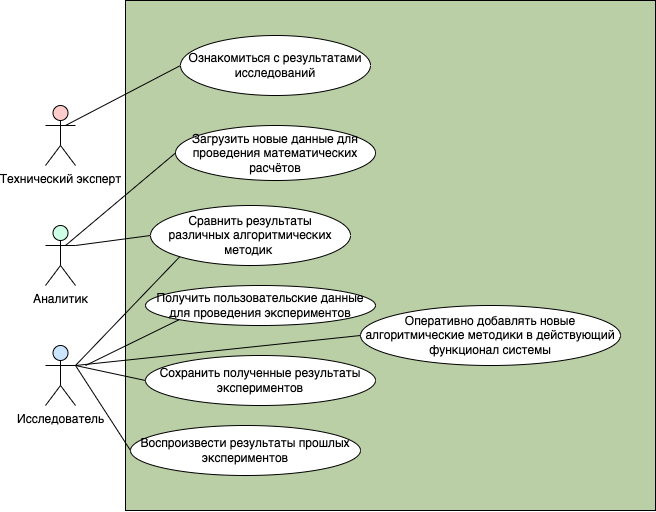
\includegraphics[width=0.6\textwidth, left]{analysis/pictures/usecases/usecase}
	\caption{Диаграмма вариантов использования}
	\label{pic:analysis__usecases-usecase}
\end{figure}
\vskip 5 mm

